%----------------------------------------------------------------------------
\appendix
%----------------------------------------------------------------------------
\chapter*{\fuggelek}\addcontentsline{toc}{chapter}{\fuggelek}
\setcounter{chapter}{\appendixnumber}
%\setcounter{equation}{0} % a fofejezet-szamlalo az angol ABC 6. betuje (F) lesz
\numberwithin{equation}{section}
\numberwithin{figure}{section}
\numberwithin{lstlisting}{section}
%\numberwithin{tabular}{section}

\section{NES kártya alkatrész elhelyezési terve}
\label{sec:NES-components}
\subsection{Top}
\label{sec:NES-components-top}
\begin{figure}[H]
	\centering
	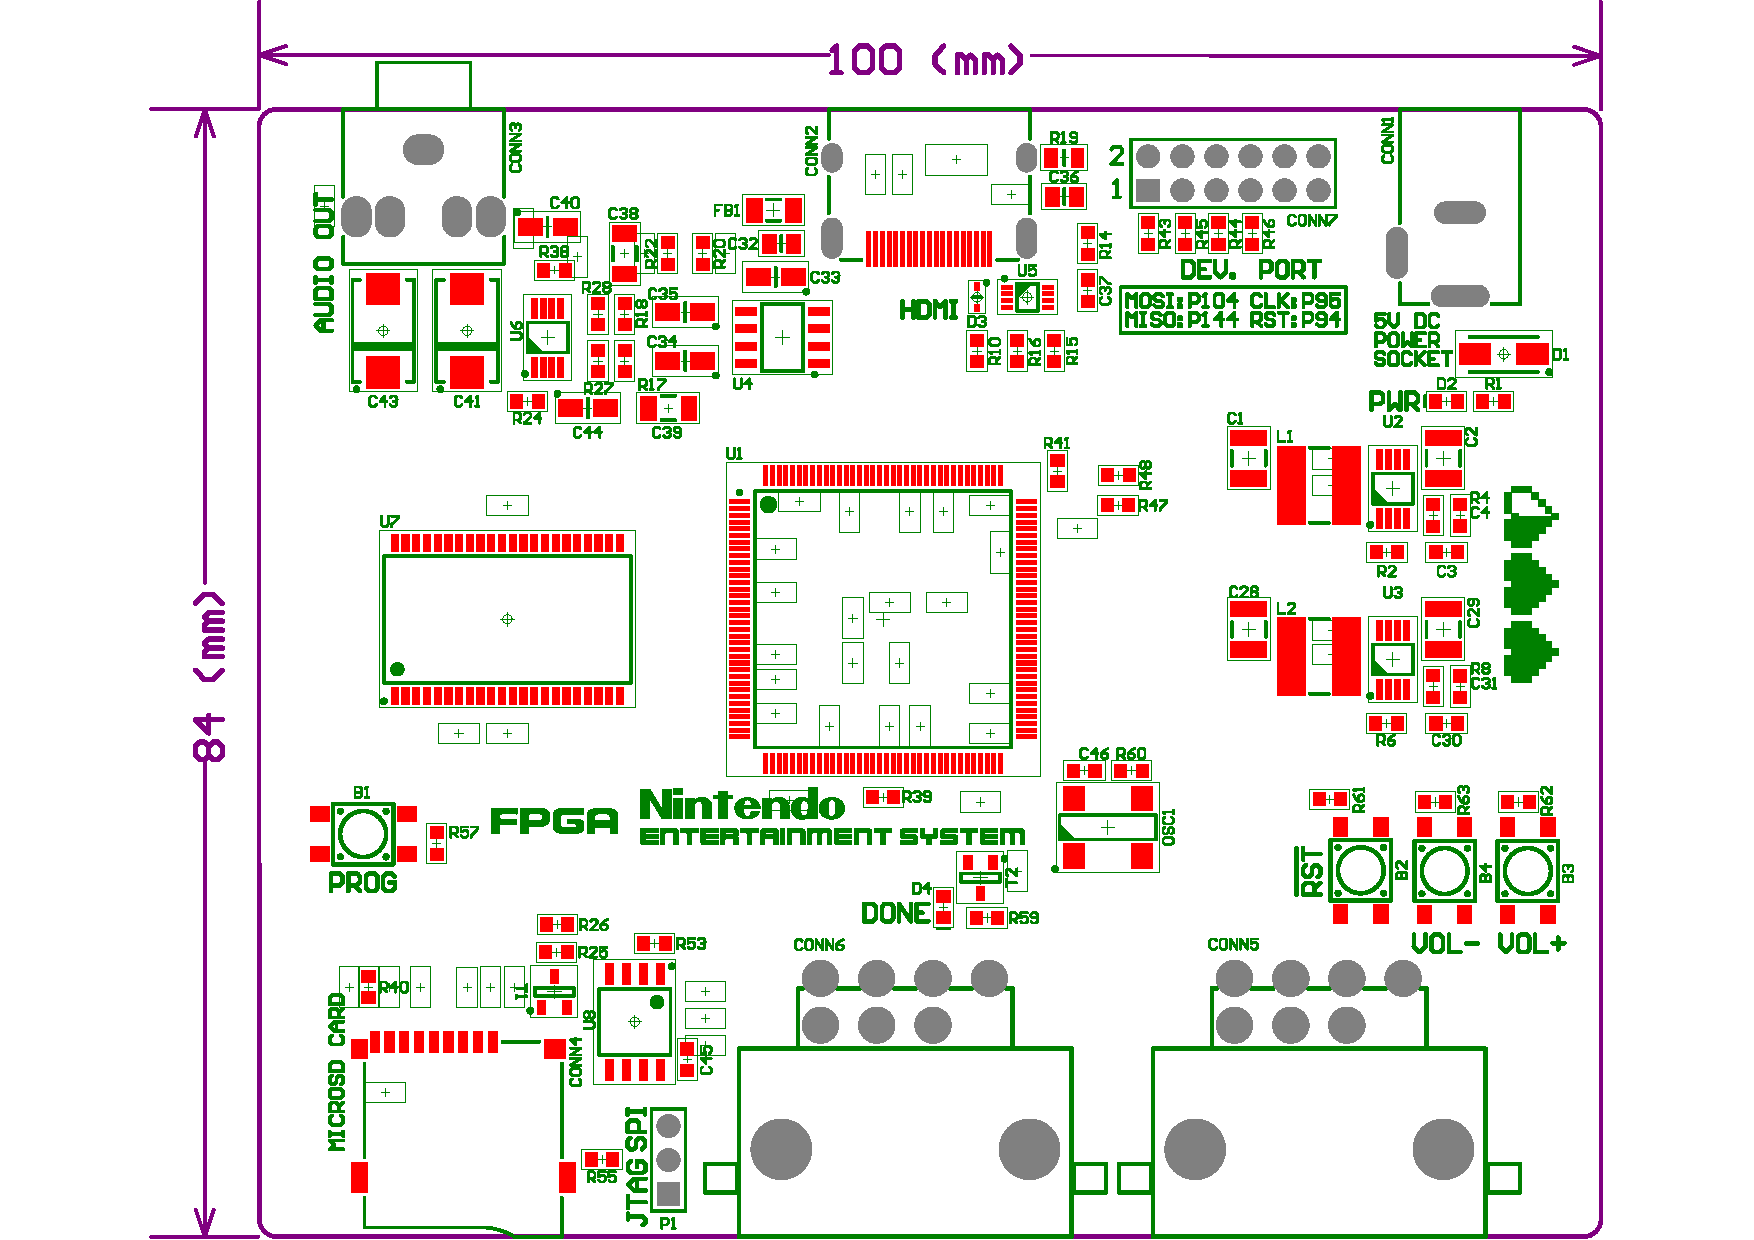
\includegraphics[width=173mm, keepaspectratio, angle=90]{figures/NES-components-top}
	
\end{figure}

\subsection{Bottom}
\label{sec:NES-components-bottom}
\begin{figure}[H]
	\centering
	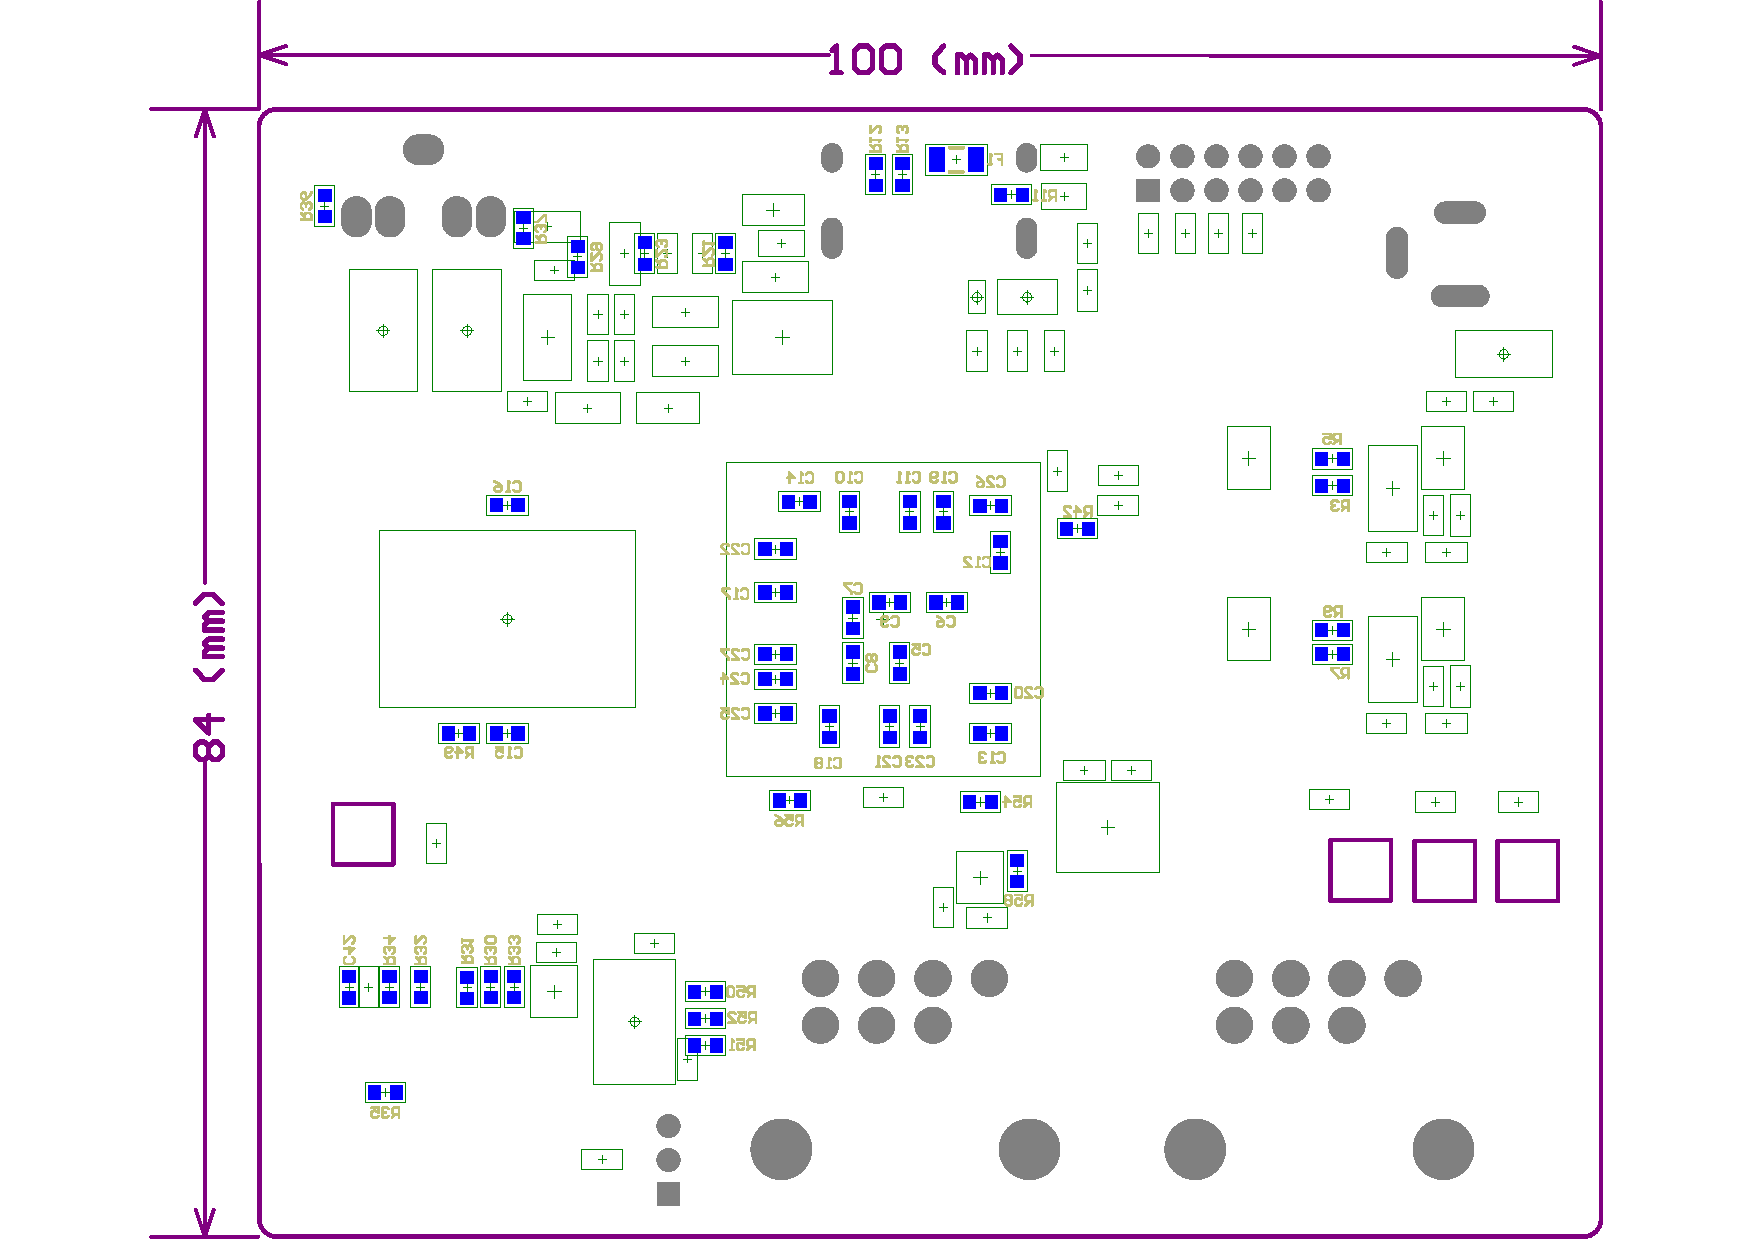
\includegraphics[width=173mm, keepaspectratio, angle=90]{figures/NES-components-bottom}
	%\caption{Tápegység} 	
\end{figure}

\section{Nyomtatott áramköri terve (2D transparent)}
\label{sec:FPGA-nes-transparency}
\begin{figure}[H]
	\centering
	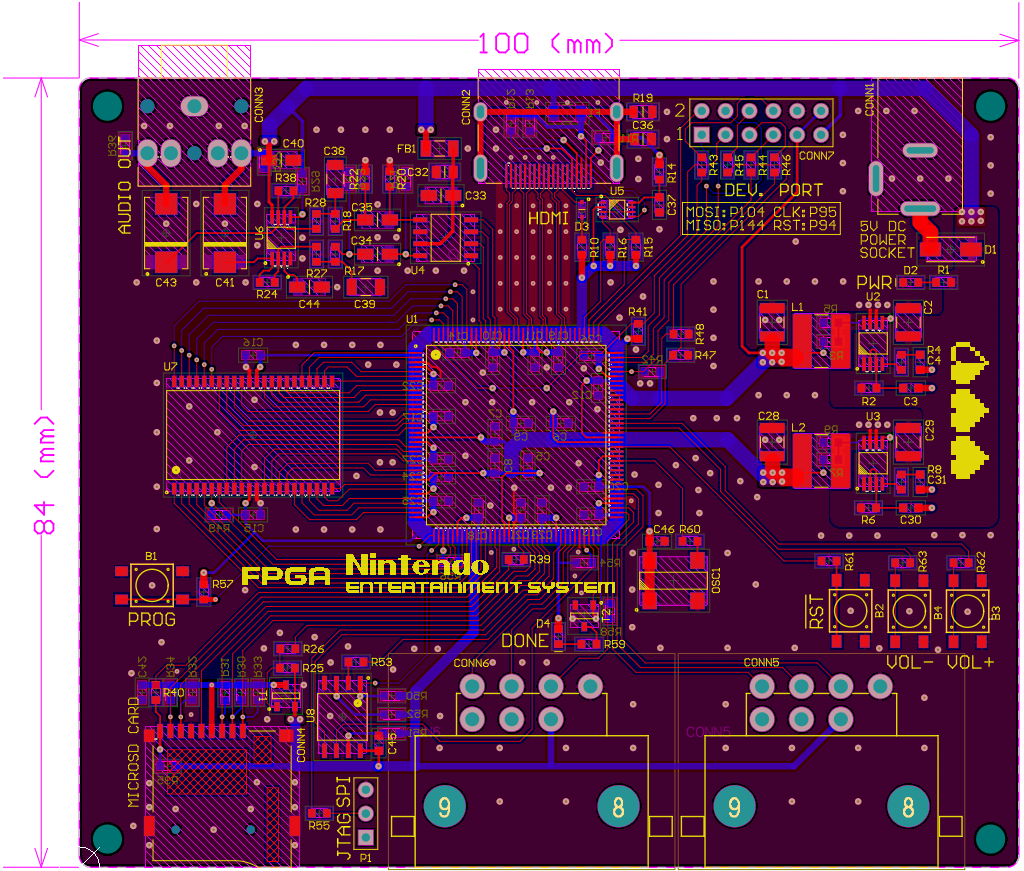
\includegraphics[width=173mm, keepaspectratio, angle=90]{figures/FPGA-nes-transparency}
	%\caption{Tápegység} 	
\end{figure}

%TODO new fugellek here
\newpage
\section{FPGA NES kártya kapcsolási rajza}
\subsection{Tápegység}
\label{sec:PSU}
\begin{figure}[H]
	\centering
	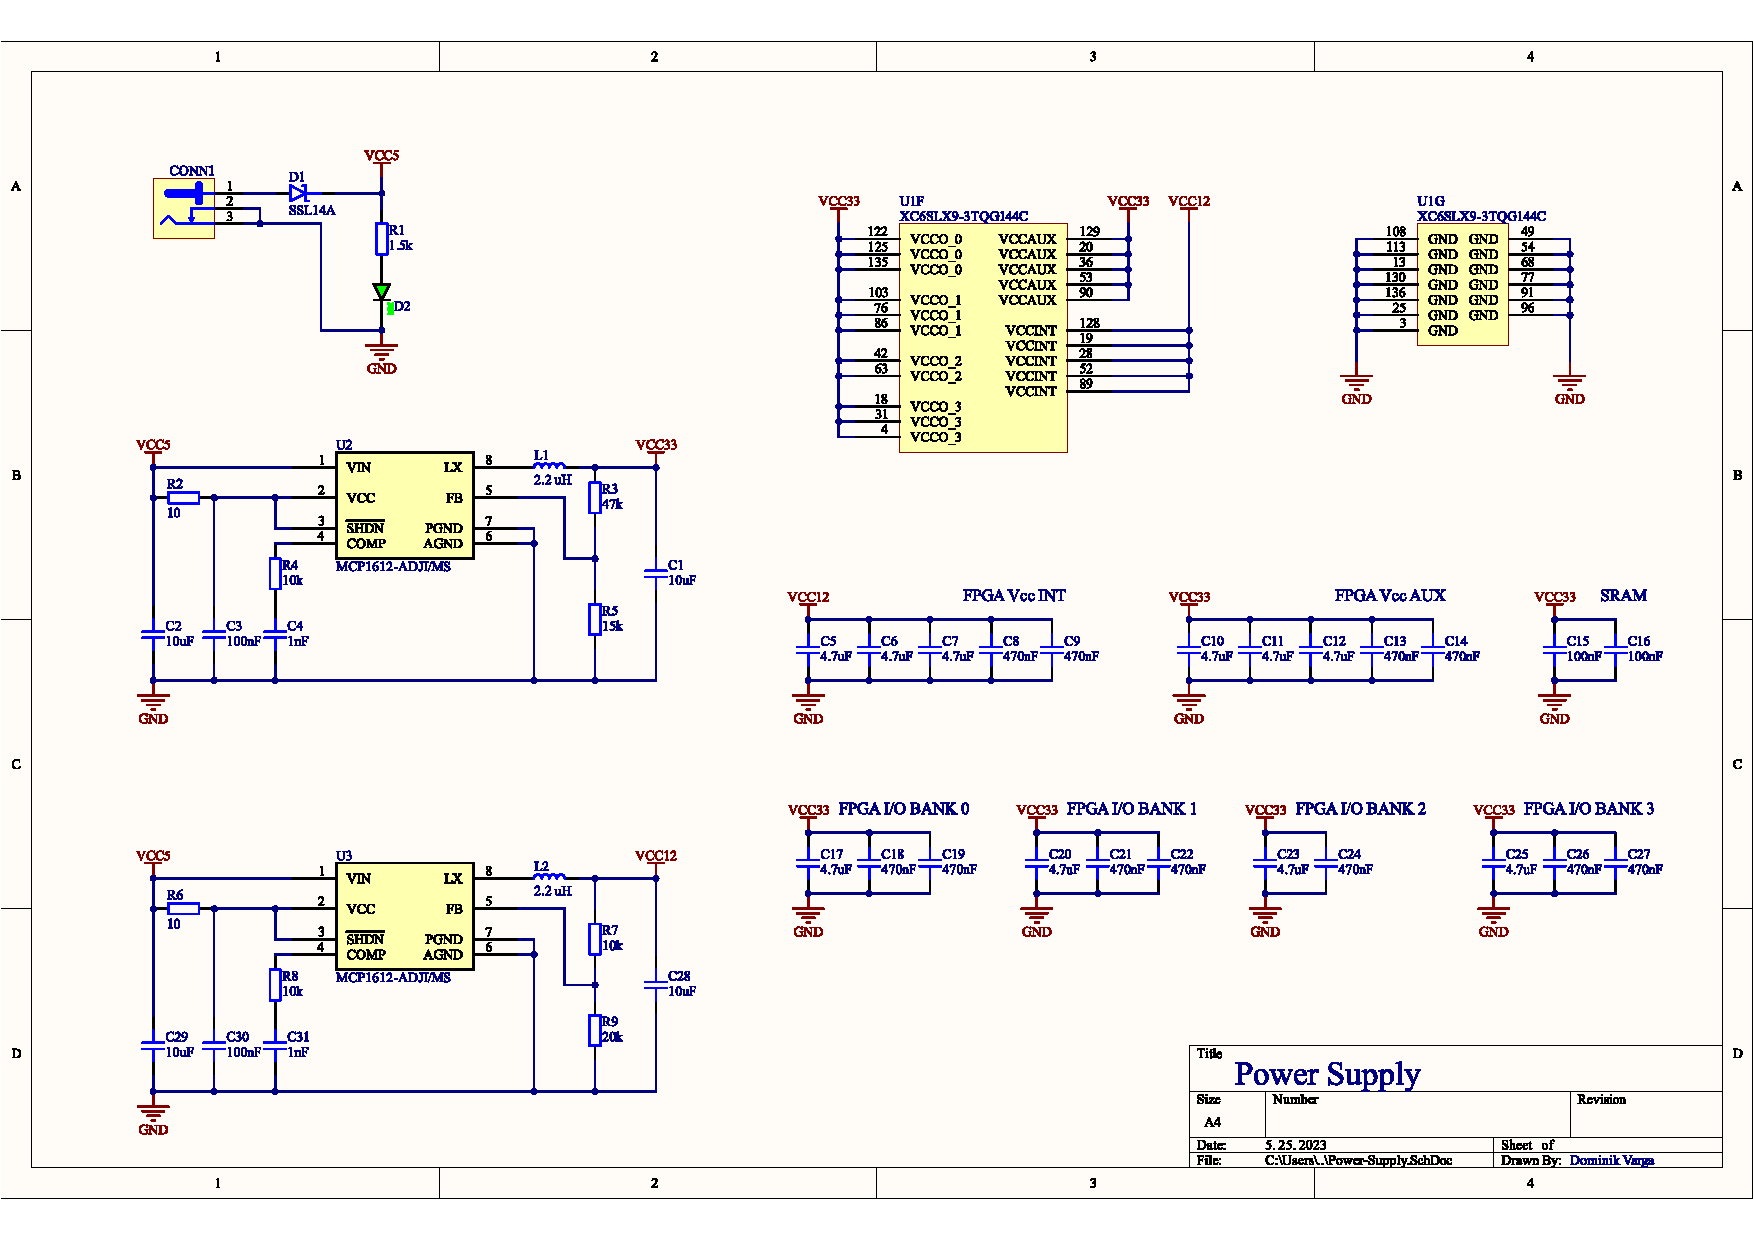
\includegraphics[width=220mm, keepaspectratio, angle=90]{figures/PSU}
	%\caption{Tápegység} 
\end{figure}
\subsection{HDMI és MicroSD kártya csatlakozó}
\label{sec:HDMI-MicroSDcard}
\begin{figure}[H]
	\centering
	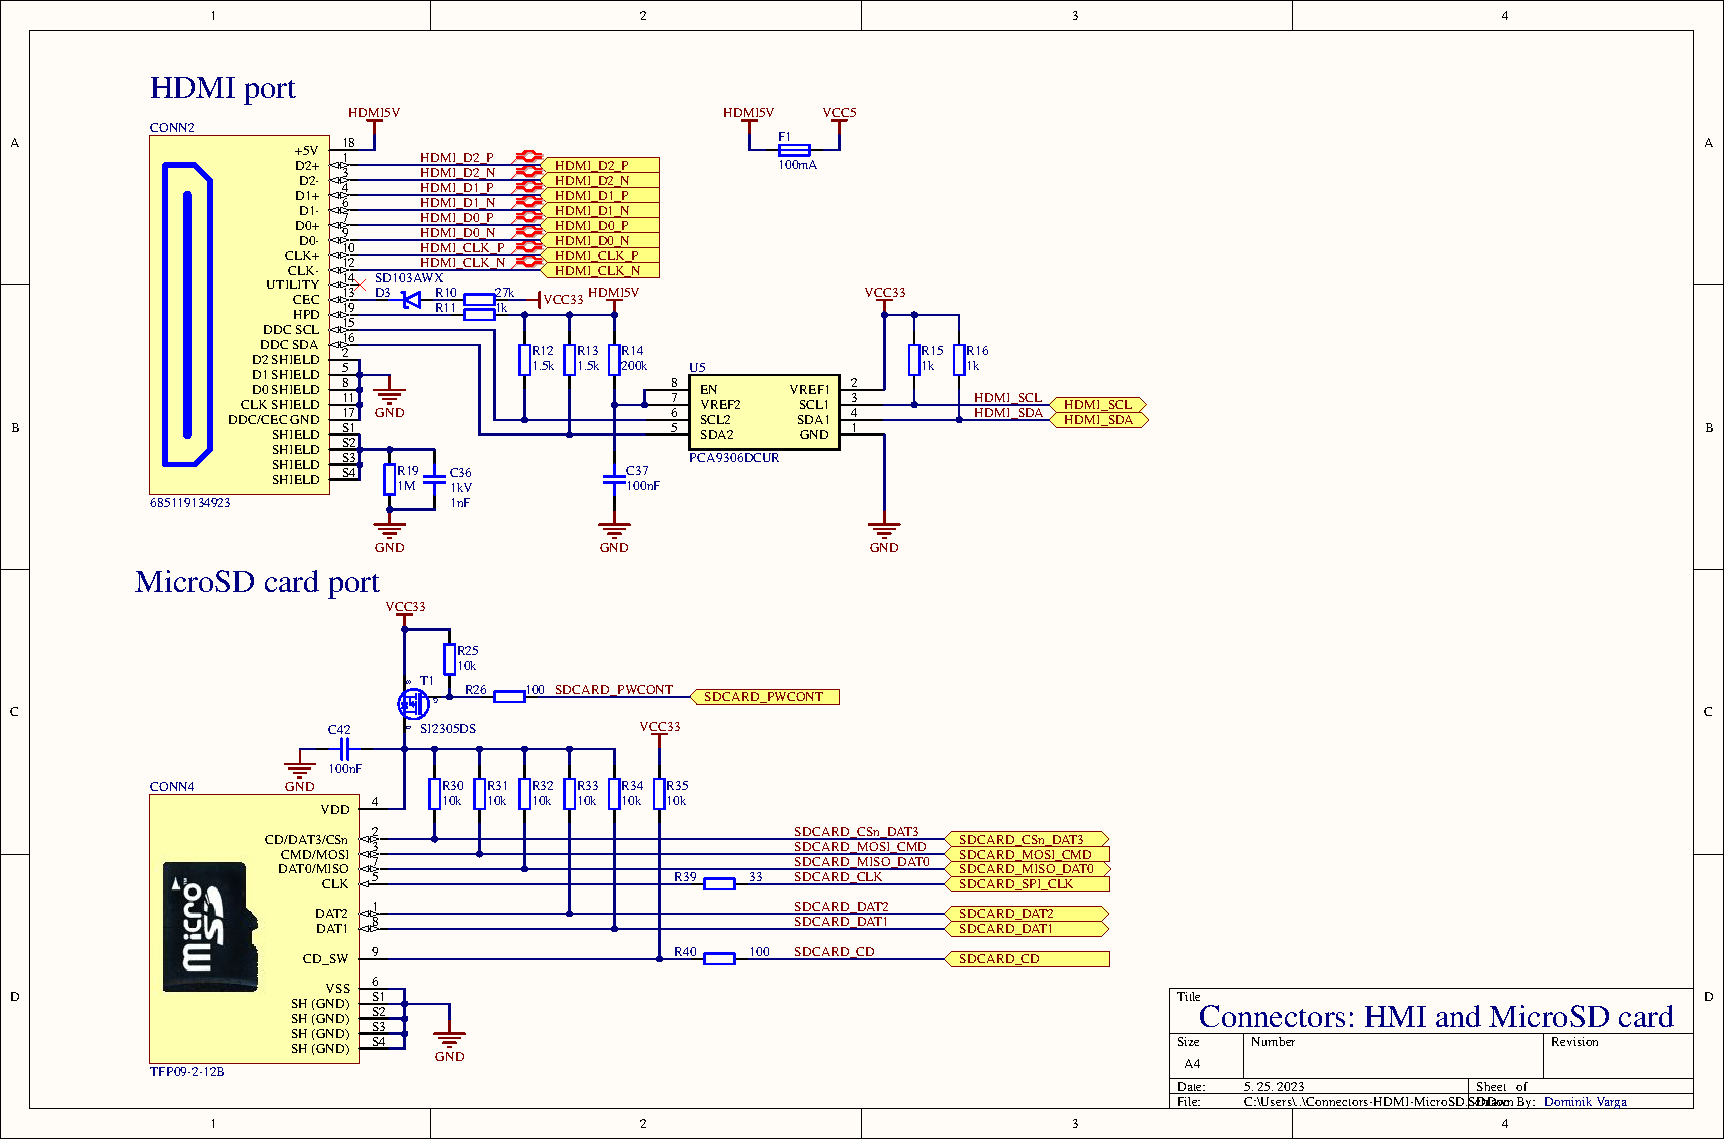
\includegraphics[width=220mm, keepaspectratio, angle=90]{figures/HDMI-MicroSDcard}
	%\caption{HDMI és MicroSD kártya csatlakozó} 
\end{figure}
\subsection{DAC, erősítő és kontroller áramkörök}
\label{sec:DAC-controllers}
\begin{figure}[H]
	\centering
	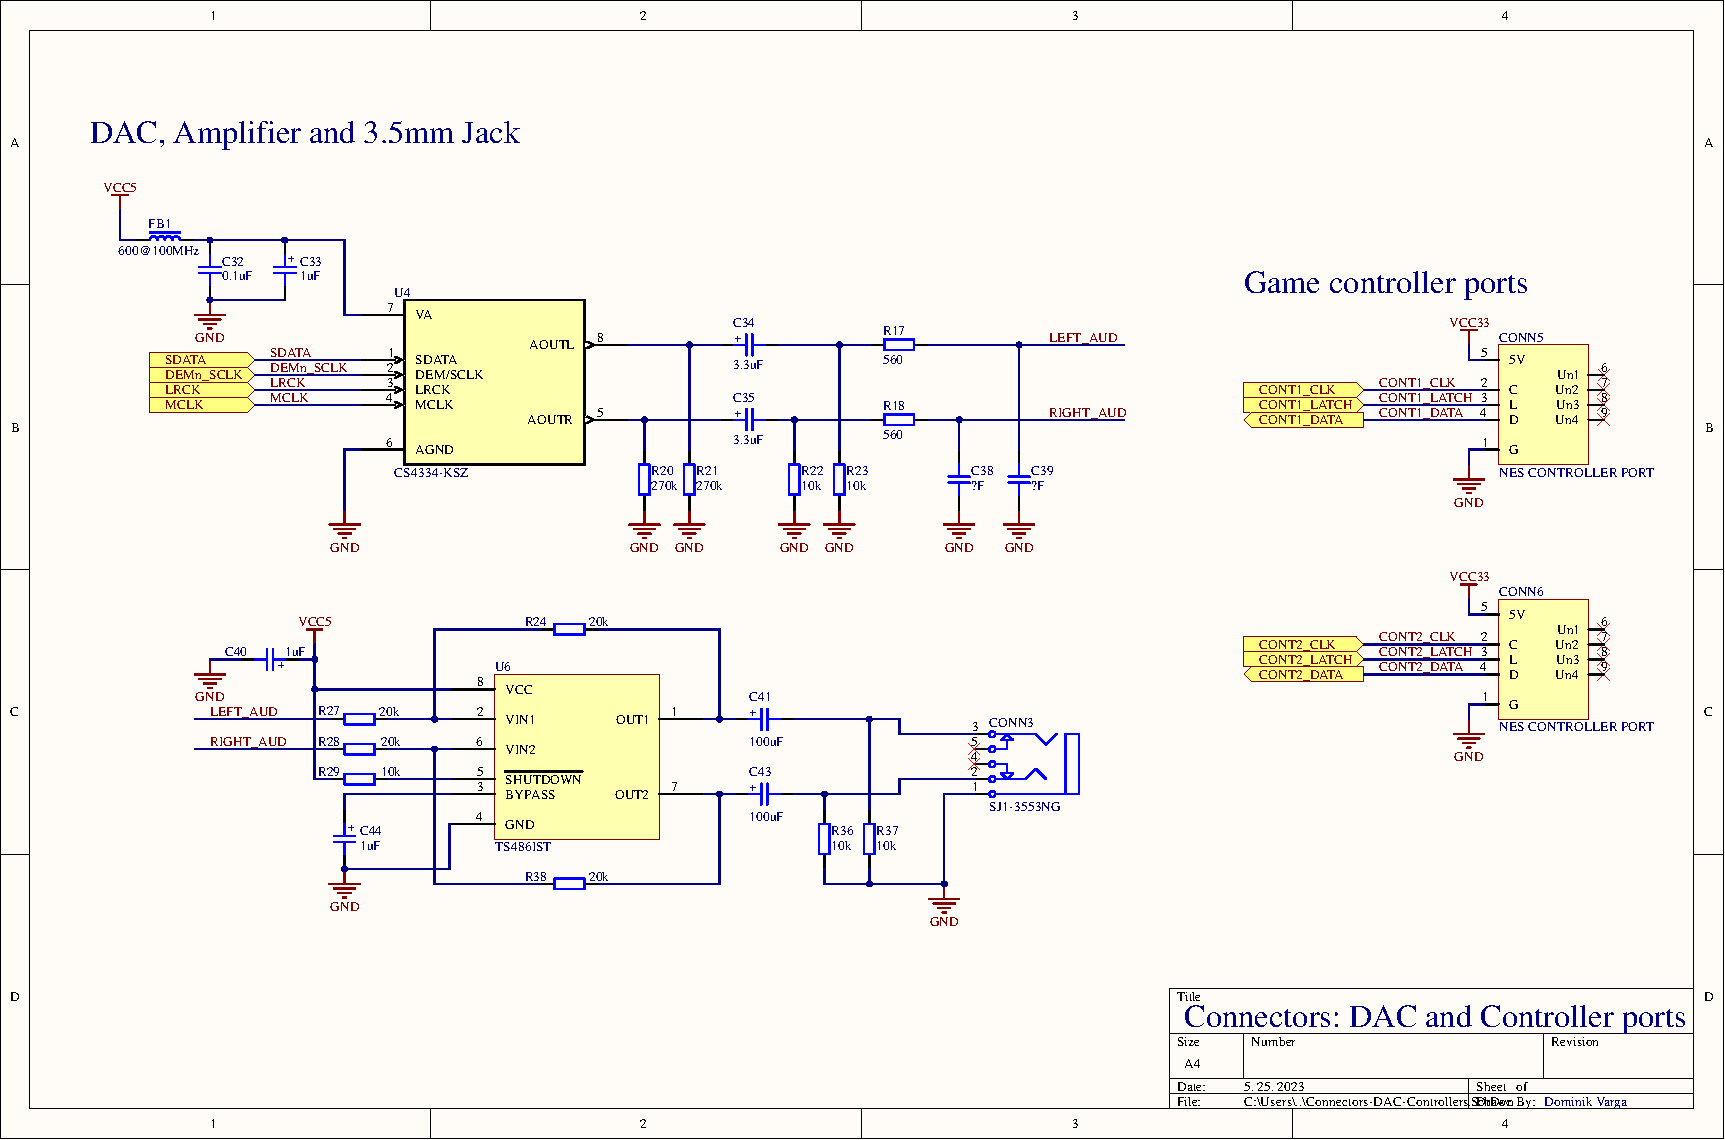
\includegraphics[width=220mm, keepaspectratio, angle=90]{figures/DAC-CONTROLLER}
	%\caption{DAC, erősítő és kontroller áramkörök}	
\end{figure}
\subsection{SRAM és SPI-Flash}
\label{sec:SRAM-SPI-Flash}
\begin{figure}[H]
	\centering
	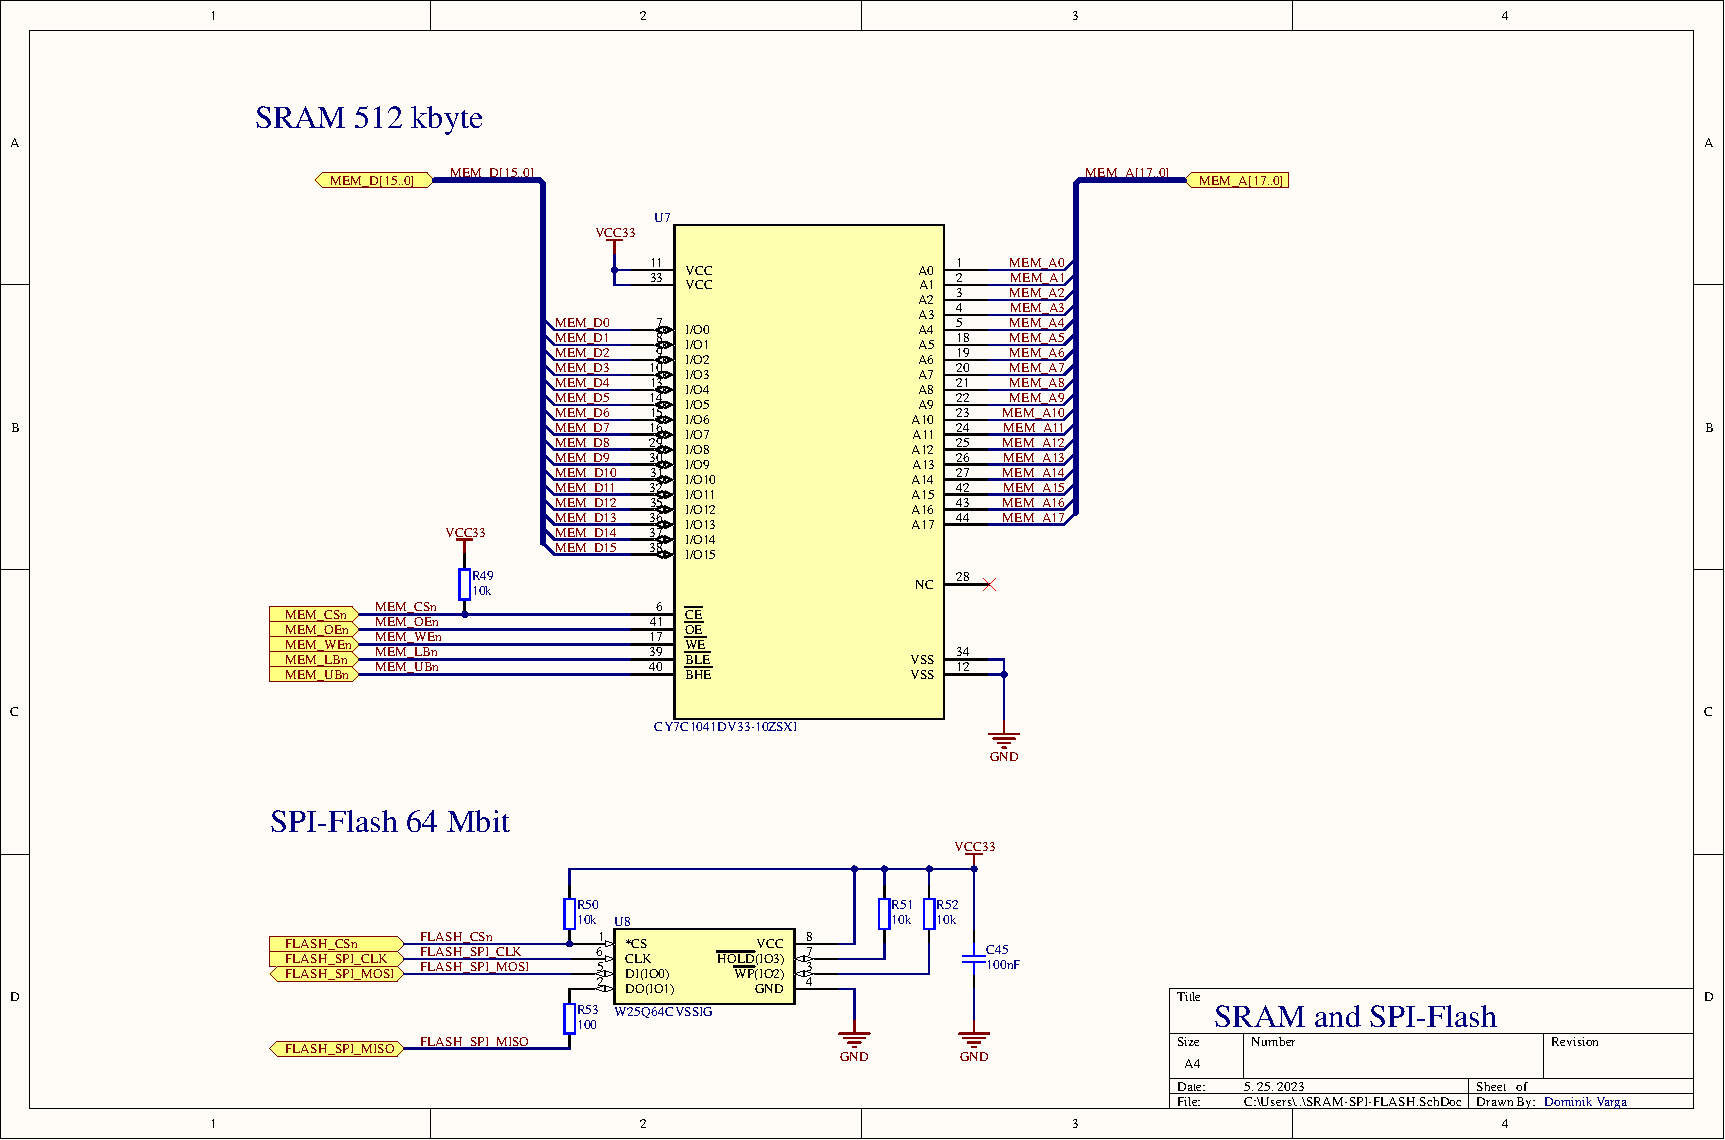
\includegraphics[width=220mm, keepaspectratio, angle=90]{figures/SRAM-FLASH}
	%\caption{SRAM és SPI-Flash} 	
\end{figure}
\subsection{FPGA OSC és JTAG}
\label{sec:OSC-JTAG}
\begin{figure}[H]
	\centering
	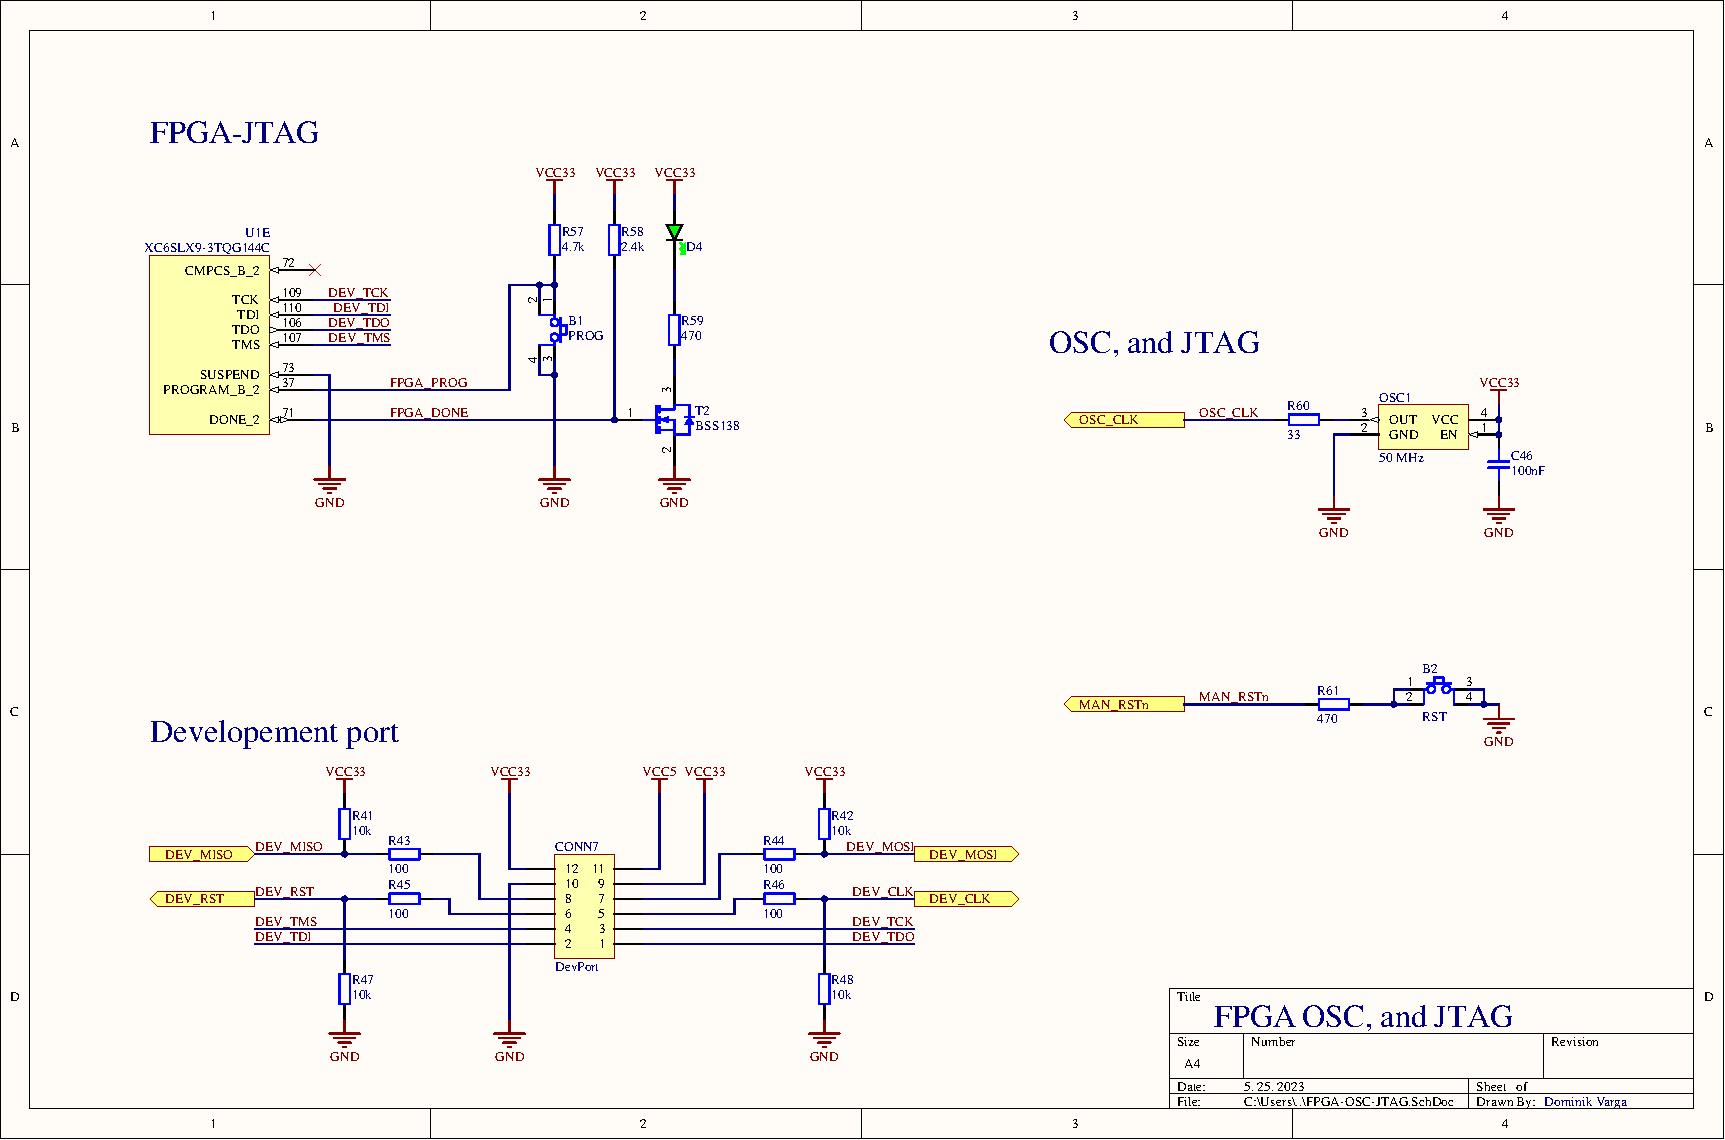
\includegraphics[width=220mm, keepaspectratio, angle=90]{figures/JTAG-OSC}
	%\caption{FPGA OSC és JTAG} 
\end{figure}
\subsection{FPGA IO bankok}
\label{sec:FPGA-BANKS}
\begin{figure}[H]
	\centering
	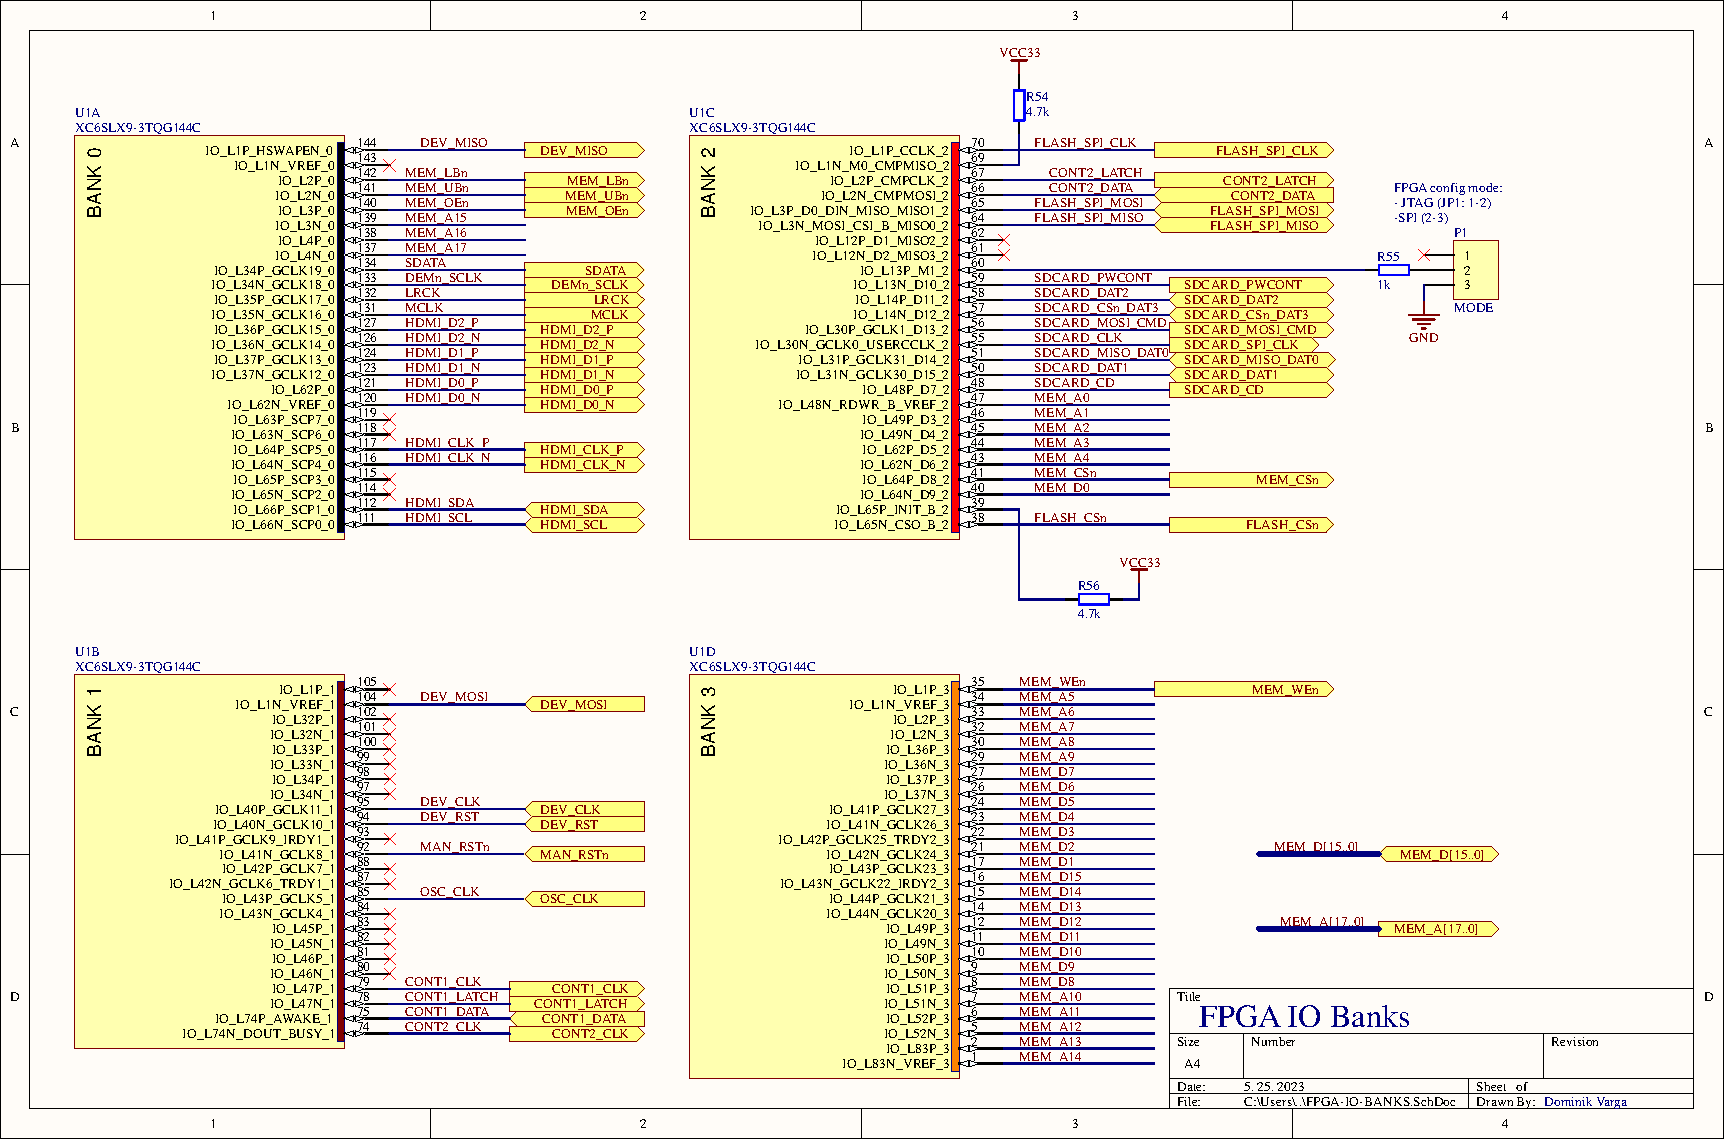
\includegraphics[width=220mm, keepaspectratio, angle=90]{figures/FPGA-BANKS}
	%\caption{FPGA IO bankok} 
\end{figure}

\newpage
\section{NTSC PPU eredeti képalkotás}
\label{sec:NTSC-PPU-frame}
\begin{figure}[H]
	\centering
	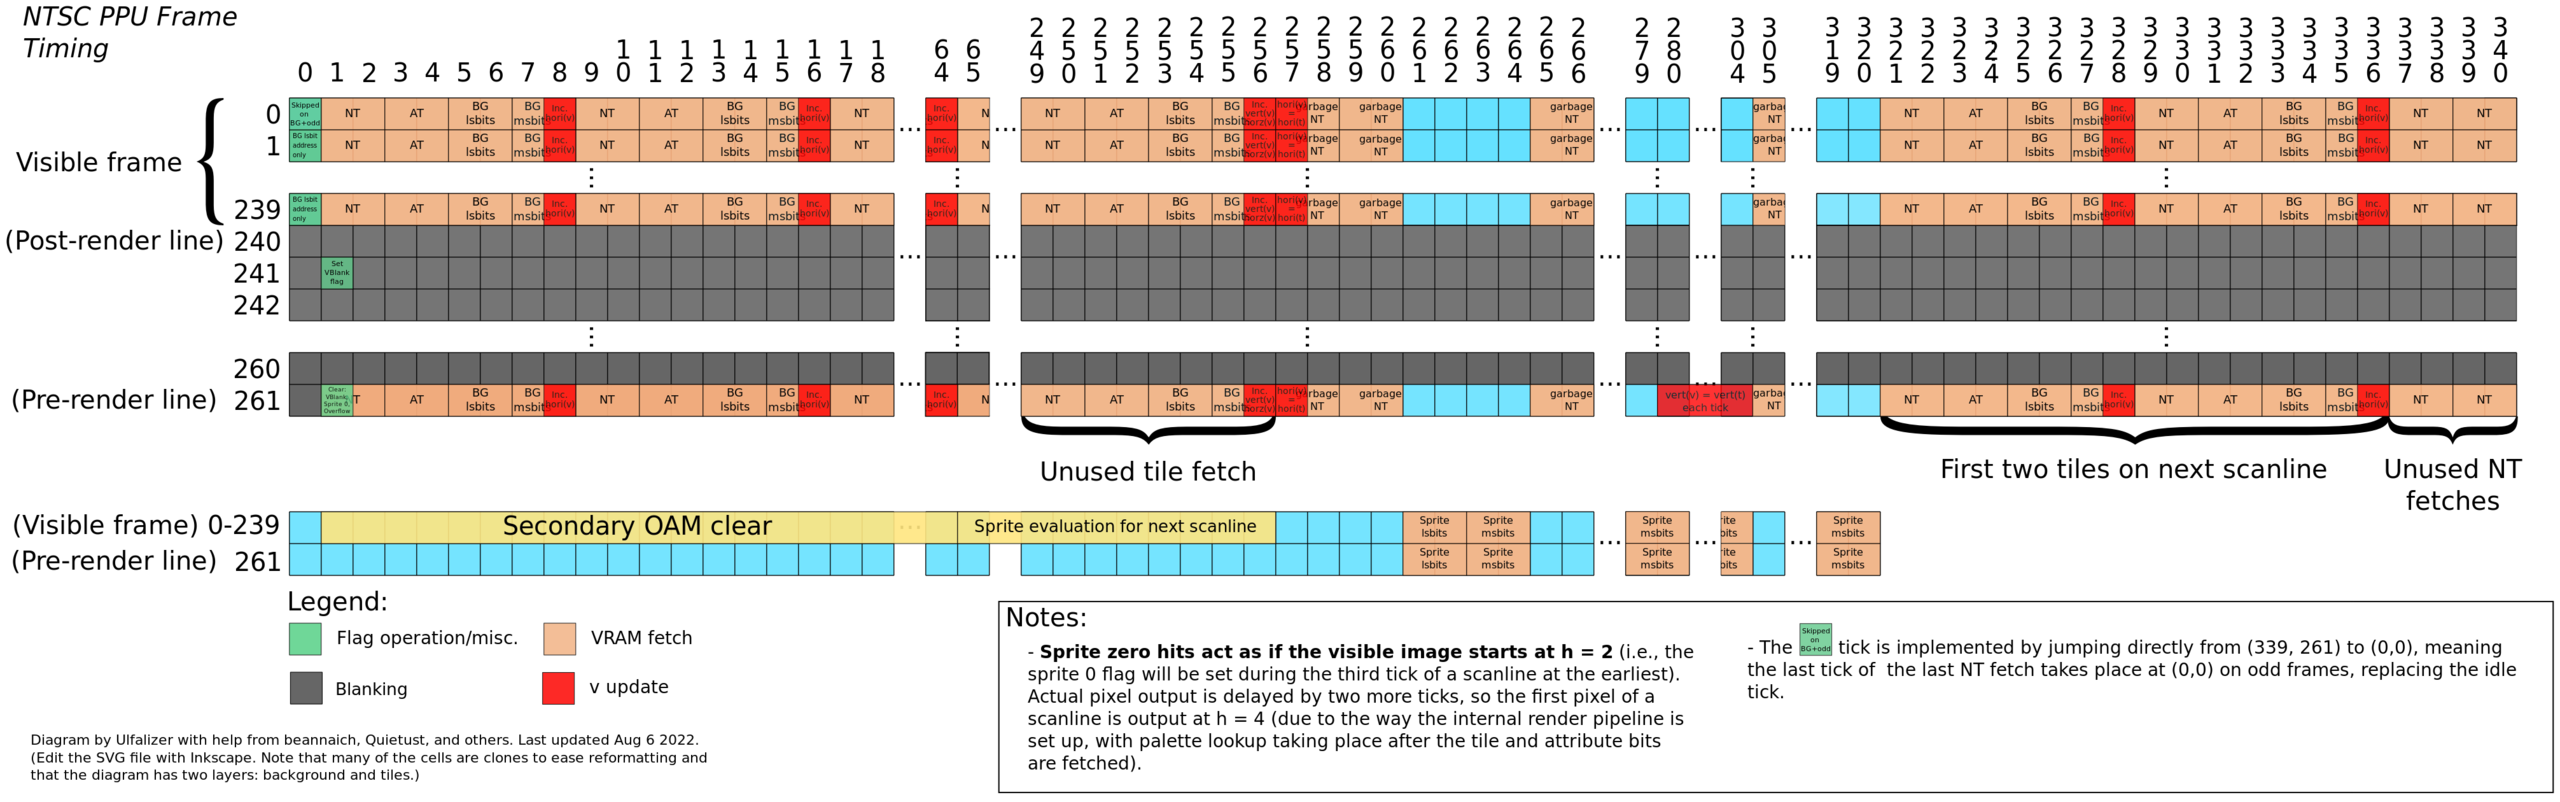
\includegraphics[width=230mm, keepaspectratio, angle=90]{figures/PPU-original-rendering}
	%\caption{FPGA IO bankok} 
\end{figure}